\chapter{First Requirement}
\section{Reading Image File}
From Reading The file, we can get the image data as a 3D array.The first dimension is the row of the pixel,The second one is the column of the pixel and the third is the RGB color channel. The value is intensity of the RGB color which varies from 0 to 255.
\vspace{20pt}
\lstinputlisting[language=Python,caption={Getting Image Data.}]{readingAudio.py}
\begin{figure}[h]
    \centering
    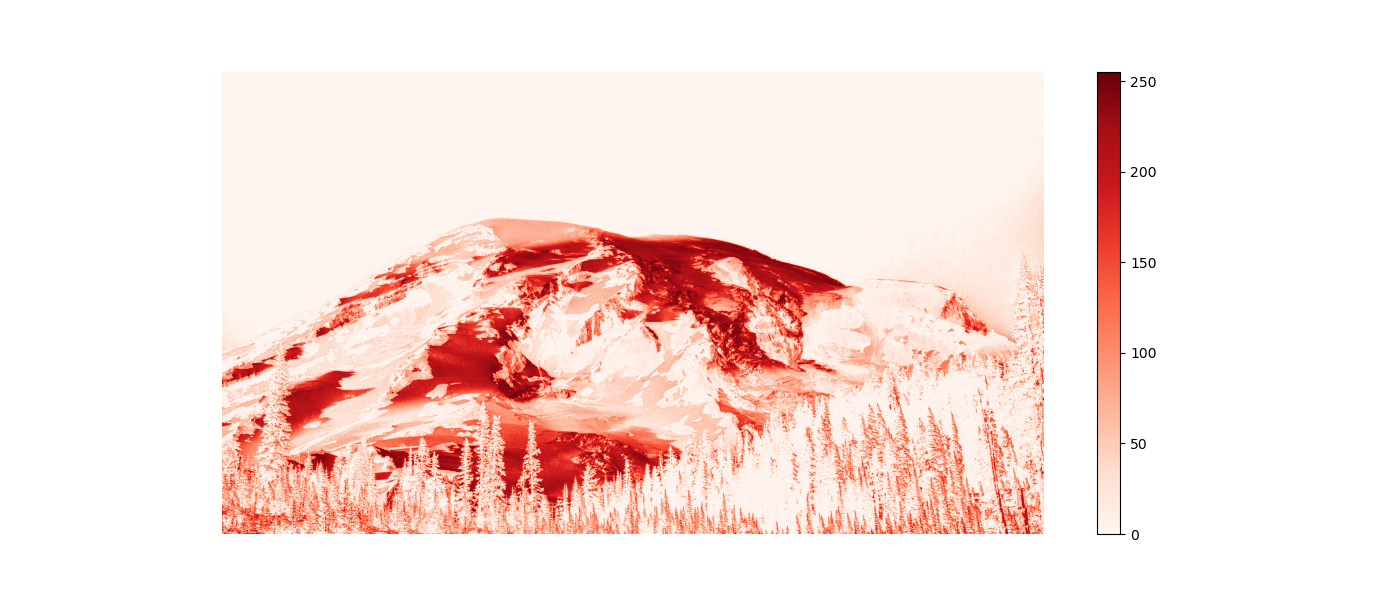
\includegraphics[width=1\textwidth]{"../Image Components/a_red.png"}
    \caption{Red component of Image.}
    \label{fig:red_component_plot}
\end{figure}
\begin{figure}[h]
    \centering
    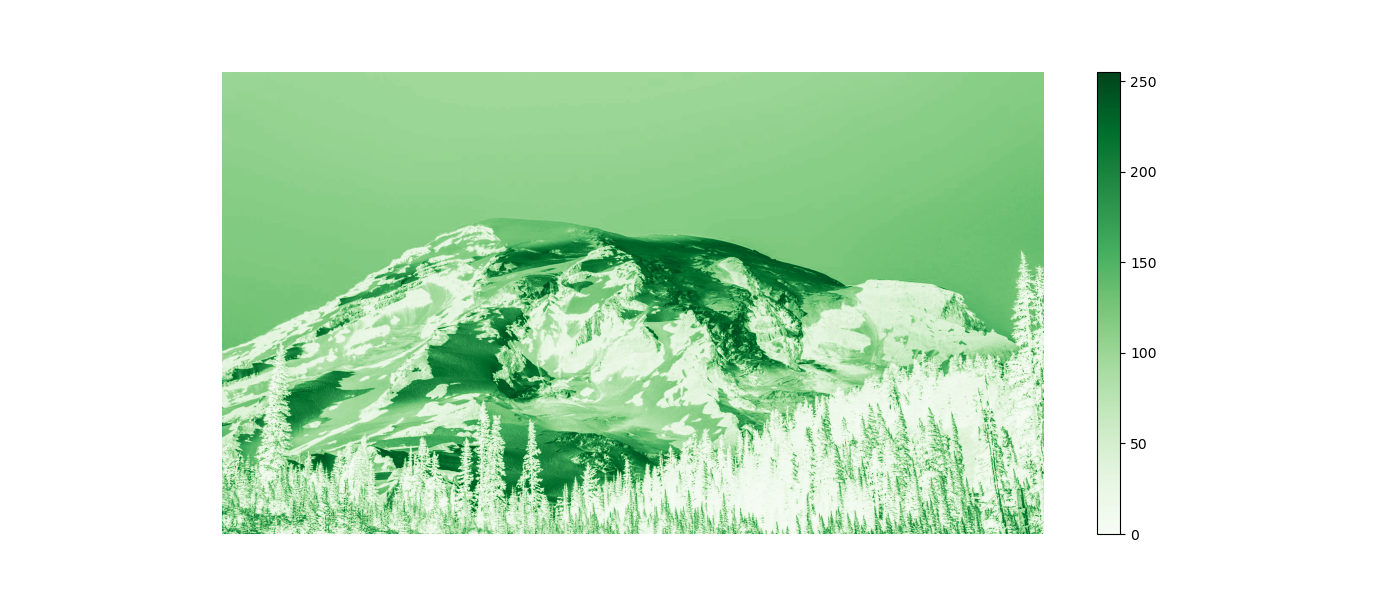
\includegraphics[width=1\textwidth]{"../Image Components/a_green.png"}
    \caption{Green component of Image.}
    \label{fig:green_component_plot}
\end{figure}
\begin{figure}[h]
    \centering
    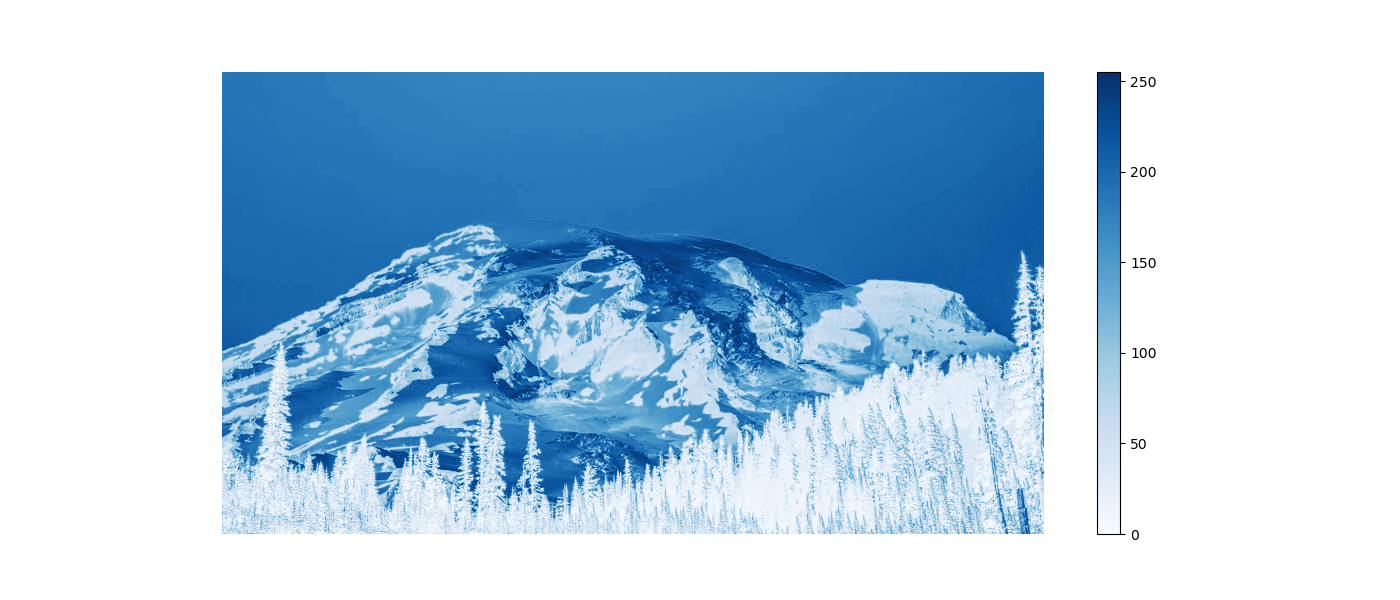
\includegraphics[width=1\textwidth]{"../Image Components/a_blue.png"}
    \caption{Blue component of Image.}
    \label{fig:blue_component_plot}
\end{figure}